Every chapter so far assumes access to a scalar reward signal: dynamic programming requires $r(s,a)$, model-free RL observes $r_t$ after each transition, and the Bellman optimality equation presupposes that rewards are known or observable. When they are neither, the DP/RL machinery cannot be applied directly.

In many domains, scalar rewards are unavailable but ordinal preferences over trajectories are easy to elicit. A human evaluator cannot assign a meaningful numerical score to a paragraph of text, but can reliably say ``response A is better than response B.'' The raw data is a set of trajectory pairs with binary preference labels. Reinforcement learning from human feedback (RLHF) uses these ordinal comparisons to learn a proxy reward function $r_\theta$, which then serves as the scalar signal for standard RL optimization. This is not an inverse problem in the IRL sense; the goal is not to rationalize observed behavior, but rather a two-stage forward problem in which the analyst first learns a reward from human judgments and then solves the resulting MDP. \citet{christiano:2017} demonstrated that this approach could train agents without an explicit reward function. RLHF has since become the predominant method for aligning large language models.

\subsection{Learning Rewards from Preferences}

The canonical RLHF framework is built on a formal model of human preference. The observed data consists of tuples $(s, y_w, y_l)$, where $s$ is a context, and $y_w$ and $y_l$ are two outputs, with $y_w$ being the ``winner'' preferred by a human. Assuming preferences follow a latent utility model, the Bradley-Terry model \citep{bradley1952rank} gives the probability that $y_w$ is preferred: $P(y_w \succ y_l | s) = \sigma(r_\theta(s, y_w) - r_\theta(s, y_l))$, where $r_\theta: \mathcal{S} \times \mathcal{Y} \to \mathbb{R}$ is a learned \textit{reward model} parameterized by $\theta$, trained to approximate human preferences (not the ground-truth reward, which is unobserved), and $\sigma(\cdot)$ is the logistic function. This formulation is a binary logit model (Section~\ref{section:language}, Equation~\ref{eq:softmax_logit}).\footnote{\citet{iskhakov2021} discuss the contrasts and synergies between machine learning and structural econometrics, including the shared reliance on logit-based choice models that underlies both RLHF and dynamic discrete choice estimation.} The reward model parameters $\theta$ are estimated by minimizing the negative log-likelihood of the observed human choices:
\begin{equation}
    \mathcal{L}(\theta) = -\mathbb{E}_{(s, y_w, y_l) \sim \mathcal{D}} \left[ \log \sigma \left( r_\theta(s, y_w) - r_\theta(s, y_l) \right) \right],
\label{eq:rlhf_loss}
\end{equation}
In the LLM setting, the ``outputs'' $y_w$ and $y_l$ are token sequences, i.e., trajectories of the autoregressive policy\footnote{An \emph{autoregressive} language model generates text token by token: at each step it outputs a distribution over the vocabulary conditioned on all preceding tokens, then samples the next token; the full response is therefore a trajectory in token space and the model acts as a sequential policy over a vocabulary-sized action set.}, so preferences are over trajectories rather than single actions. The preference loss in Equation~(\ref{eq:rlhf_loss}) is MLE of a choice model where the ``alternatives'' are trajectory segments and the ``choice'' is the human-preferred one.

This logit foundation is also a social-choice assumption once labelers are heterogeneous. Pooling pairwise comparisons from many evaluators does not recover a neutral ``human preference''; it estimates a single score whose odds ratios summarize the aggregation rule induced by the sampling scheme, label model, and loss function. Recent alignment work makes this point explicit. Standard Bradley-Terry-style reward learning can behave like a hidden social welfare function, can fail natural axioms for aggregating rankings, and can create strategic reporting incentives when preferences differ across contexts or groups \citep{conitzer2024socialchoice,siththaranjan2024distributional,ge2024axioms,park2024heterogeneous}. DPO inherits the same aggregation problem because it replaces the explicit reward model with an implicit reward difference, not with a theory of whose preferences count.

\subsection{The RLHF Pipeline and Direct Optimization}

The learned $r_\theta$ then serves as a proxy objective for policy optimization. Building on the reward-learning and RL fine-tuning framework of \citet{ziegler2019fine} and \citet{stiennon2020learning}, the canonical three-stage pipeline was formalized by \citet{ouyang2022training}. First, a base pretrained model is initialized via supervised fine-tuning (SFT)\footnote{\emph{Pretraining} optimizes a language model to predict the next token across a massive text corpus, producing broad linguistic knowledge with no behavioral objective. \emph{Supervised fine-tuning} (SFT) continues training on a small curated dataset of (prompt, ideal-response) pairs to specialize the model toward the desired task and establish the reference policy $\pi^{SFT}$ from which the KL penalty is measured.} on a small dataset of high-quality demonstrations, yielding an initial policy $\pi^{SFT}$. This grounds the model in the desired style and format. The second step is the reward model training as described, using preference data generated from this $\pi^{SFT}$.

In the third step, the SFT policy $\pi_\phi$ is fine-tuned via PPO (Section~\ref{sec:actor_critic}) to maximize the frozen reward model $r_\theta$,\footnote{After fine-tuning concludes, the reward model may be reused for evaluation or for later alignment iterations, but it is not updated inside the PPO optimization loop.} with a KL-divergence penalty preventing the policy from drifting into regions where $r_\theta$ is unreliable. The objective is
\begin{equation}
    J(\phi) = \mathbb{E}_{s \sim \mathcal{D}, y \sim \pi_\phi(\cdot|s)} [r_\theta(s, y)] - \lambda_{KL} \mathbb{E}_{s \sim \mathcal{D}} [D_{KL}(\pi_\phi(\cdot|s) \,||\, \pi^{SFT}(\cdot|s))],
\label{eq:rlhf_objective}
\end{equation}
where $D_{KL}$ is the Kullback-Leibler divergence and $\lambda_{KL}$ controls the penalty strength.\footnote{$\lambda_{KL}$ denotes the KL penalty weight, reserving $\beta$ for model parameters and $\gamma$ for discount factors. The standard RLHF literature, including \citet{rafailov2023direct}, uses $\beta$ for this parameter.} Without this constraint, the policy exploits inaccuracies in $r_\theta$ to achieve high proxy scores with degenerate behavior (``reward hacking''), the RLHF analogue of divergence under function approximation (Section~\ref{sec:deadly_triad}).

The KL-regularized objective in Equation~(\ref{eq:rlhf_objective}) admits a Bayesian interpretation \citep{korbak2022rl}. In this view, the reference policy $\pi^{SFT}$ acts as a prior distribution over plausible responses. The reward model $r_\theta$ provides evidence, specifying which responses are more desirable. The goal of alignment is to find the posterior distribution $\pi^*$ that optimally combines the prior with this evidence. This ideal posterior policy takes the form of Equation~(\ref{eq:rlhf_posterior}):
\begin{equation}
    \pi^*(y|s) \propto \pi^{SFT}(y|s) \exp\left(\frac{r_\theta(s, y)}{\lambda_{KL}}\right).
\label{eq:rlhf_posterior}
\end{equation}
The reward function scaled by $\lambda_{KL}$ defines the log-likelihood, so the KL-regularized objective $J(\phi)$ is equivalent (up to an additive constant) to the Evidence Lower Bound (ELBO) for this Bayesian inference problem. Maximizing the RLHF objective via PPO is therefore variational inference: finding the policy $\pi_\phi$ that minimizes KL divergence to $\pi^*$. This reframes the KL penalty as a structural component of the inference problem rather than an ad-hoc regularizer.

Despite this closed-form characterization, the three-stage RLHF pipeline is complex to implement, requiring training multiple large models and a computationally expensive RL loop. Direct Preference Optimization (DPO), introduced by \citet{rafailov2023direct}, collapses the pipeline into a single supervised learning objective by reparameterizing the reward function in terms of $\pi^*$ and $\pi^{SFT}$, as in Equation~(\ref{eq:dpo_reparameterize}):
\begin{equation}
    r(s,y) = \lambda_{KL} \log\left(\frac{\pi^*(y|s)}{\pi^{SFT}(y|s)}\right) + \lambda_{KL} \log Z(s).
\label{eq:dpo_reparameterize}
\end{equation}
When this analytical expression for the reward is substituted into the Bradley-Terry preference loss from Equation~(\ref{eq:rlhf_loss}), the unknown partition function $Z(s)$ cancels out. This yields a loss function that depends only on the policy $\pi_\phi$ being optimized and the fixed reference policy $\pi^{SFT}$. The DPO objective, given in Equation~(\ref{eq:dpo_loss}), is thus a simple binary cross-entropy loss over policy likelihoods:
\begin{equation}
    \mathcal{L}_{DPO}(\phi; \pi^{SFT}) = -\mathbb{E}_{(s, y_w, y_l) \sim \mathcal{D}} \left[ \log \sigma \left( \lambda_{KL} \log \frac{\pi_\phi(y_w|s)}{\pi^{SFT}(y_w|s)} - \lambda_{KL} \log \frac{\pi_\phi(y_l|s)}{\pi^{SFT}(y_l|s)} \right) \right].
\label{eq:dpo_loss}
\end{equation}
This objective is optimized on $\phi$ using standard supervised learning with a static preference dataset. The gradient increases the likelihood of preferred responses $y_w$ and decreases the likelihood of dispreferred responses $y_l$, relative to the reference policy.

The growing family of DPO variants is best read economically by asking what part of the preference problem changes. IPO modifies the link/objective structure to avoid some DPO overfitting behavior \citep{azar2024preferenceparadigm}. KTO replaces pairwise comparisons with a prospect-theory-style objective over desirable and undesirable outputs \citep{ethayarajh2024kto}. Nash-LHF and SPPO treat preference optimization as a game over pairwise comparisons, which is closer to social choice when preferences are cyclic or non-transitive \citep{munos2023nash,wu2024sppo}. MaxMin-RLHF makes the aggregation rule explicitly egalitarian \citep{chakraborty2024maxmin}. ORPO, SimPO, and robust DPO mainly change implementation, reference-model dependence, or noisy-label bias rather than the underlying welfare question \citep{hong2024orpo,meng2024simpo,chowdhury2024rdpo}. Self-rewarding loops move some feedback generation from humans to model judges, which lowers data-collection costs but makes the evaluator itself part of the mechanism \citep{yuan2024self}.

\begin{figure}[t]
\centering
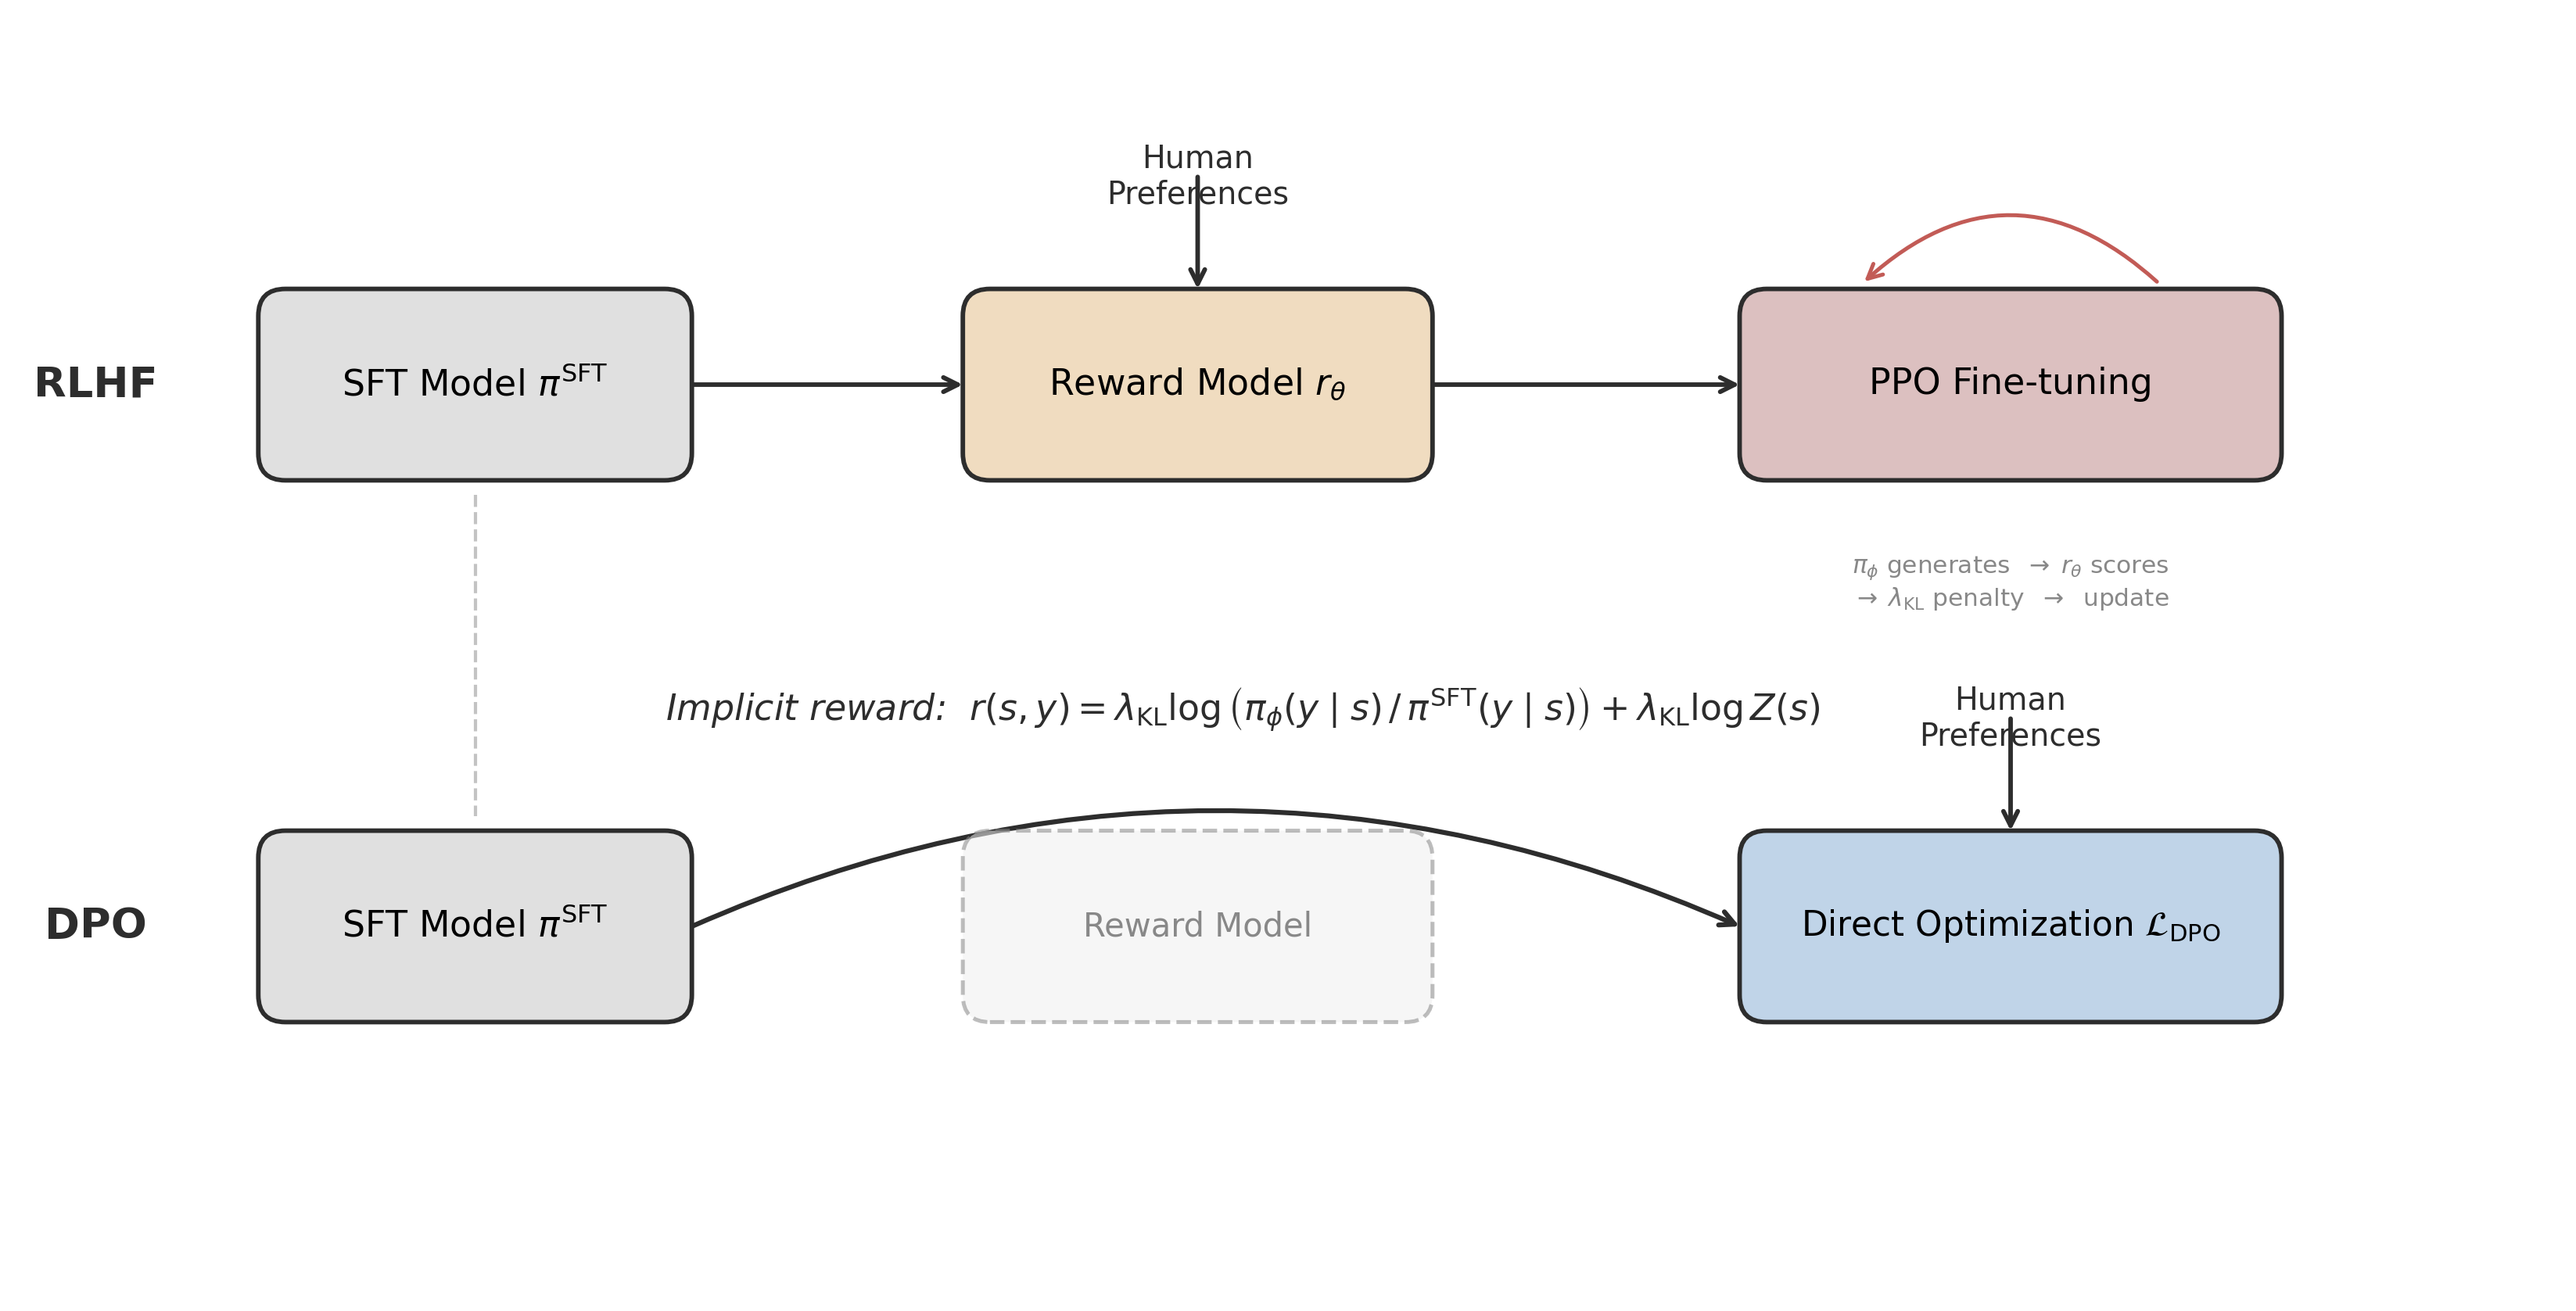
\includegraphics[width=\textwidth]{../ch09_rlhf/sims/rlhf_dpo_pipeline.png}
\caption[RLHF versus DPO pipelines]{RLHF versus DPO pipelines. Top row: the three-stage RLHF pipeline trains a reward model from human preferences, then uses PPO to fine-tune the policy with a KL penalty. Bottom row: DPO collapses the pipeline into a single supervised learning objective over preference pairs, eliminating the explicit reward model (ghosted box).}
\label{fig:rlhf_dpo_pipeline}
\end{figure}

\subsection{Social Choice and Whose Preferences}
\label{sec:social_choice}

RLHF turns alignment into an economics problem: elicit preferences, aggregate them across people, design incentives for truthful feedback, and interpret the learned object. The phrase ``alignment tax'' appears in the assistant-alignment literature as a warning that optimizing for helpfulness, harmlessness, and honesty can trade off against other capabilities \citep{askell2021general}; \citet{ouyang2022training} provide concrete InstructGPT evidence of benchmark regressions on tasks such as SQuAD, DROP, and HellaSwag. That evidence is an empirical frontier of a particular training recipe, model class, and evaluation set, not a fundamental constraint.

The central welfare question is whose preferences are being aligned to. If one reward model is trained on pooled labels from a non-representative group of contractors, the resulting policy optimizes an implicit aggregation rule, not society's preferences. Social choice provides the concepts for this problem: alternatives, voters, ranking rules, impossibility theorems, strategic reports, minority protection, and interpersonal aggregation \citep{conitzer2024socialchoice,mishra2023socialchoice}. Distributional preference learning and axiomatic analyses show that standard BTL aggregation can encode Borda-like rules or fail desirable fairness and consistency conditions \citep{siththaranjan2024distributional,ge2024axioms}. Alternatives such as personalization, MaxMin-RLHF, Nash learning from human feedback, and maximal-lottery alignment make the aggregation rule more explicit, though some of these connections remain preprint-level rather than settled practice \citep{park2024heterogeneous,chakraborty2024maxmin,munos2023nash,maurarivero2025maximal}.

\subsection{Mechanism Design for Feedback}

Feedback is elicited through a mechanism, not passively observed. Labelers may be inattentive, strategic, ideologically motivated, or selected by the platform's contracting process. Mechanism design therefore enters before the reward model is trained. VCG-style fine-tuning formulations ask how to aggregate multiple reward models when participants can benefit from manipulating the training rule \citep{sun2024mechanism}. Strategyproof RLHF studies the same issue for preference reports, with a tradeoff between incentive compatibility and the quality of the final policy \citep{kleinebuening2025strategyproof}. Older peer-prediction mechanisms such as Bayesian truth serum and output-agreement methods show how payments can elicit truthful subjective signals when no ground truth is immediately observable \citep{prelec2004bayesian,miller2005eliciting}. For RLHF, this means the data-generating process is not a nuisance detail; it determines which preferences are observed and how costly truthful feedback is.

\subsection{Structural Identification}

Finally, preference optimization is not welfare analysis unless the learned reward has a structural interpretation. Bradley-Terry and DPO identify reward differences only through observed pairwise comparisons, up to normalizations and only on the covered comparison support. IRL identification results show that many rewards can rationalize the same behavior or preferences, and that entropy regularization, extra environments, or downstream invariance restrictions are needed to recover sharper objects \citep{cao2021identifiability,skalse2023invariance,knox2022preference}. Economically, the genealogy runs from McFadden logit choice \citep{mcfadden:1973}, through Rust-style dynamic discrete choice \citep{rust1994structural,rust1996numerical}, to maximum-entropy IRL \citep{Ziebart2008}, and finally to DPO's log-odds reparameterization \citep{rafailov2023direct}. Recent econometric work makes this bridge explicit, but still as an emerging working-paper literature rather than a settled textbook synthesis \citep{vanderlaan2025efficient,Kang2025,RustRawat2026}. The practical lesson is conservative: RLHF can produce useful policies, but the reward object is partially identified, aggregation-dependent, and limited by the offline support of the comparison data.

\FloatBarrier
\subsection{Engine Replacement MDP: What Preferences Do and Do Not Identify}
\label{engine:ch09}

\begin{table}[H]
\centering
\small
\caption{DPO reward inversion on the Engine Replacement MDP at $\lambda_{KL}=0.5$. The four rows report the exponential tilt and the normalized policy. The final column is the reward representative selected by the DPO normalization.}
\label{tab:engine_preferences}
\begin{tabular}{llrrrrrr}
\hline
state & action & $r$ & $\pi^{SFT}$ & $e^{r/\lambda_{KL}}$ & $\pi^{SFT}e^{r/\lambda_{KL}}$ & $\pi^*$ & $\lambda_{KL}\log(\pi^*/\pi^{SFT})$ \\
\hline
low & keep & 1.0000 & 0.6000 & 7.3891 & 4.4334 & 0.9679 & 0.2391 \\
low & replace & -0.5000 & 0.4000 & 0.3679 & 0.1472 & 0.0321 & -1.2609 \\
high & keep & 0.2000 & 0.4000 & 1.4918 & 0.5967 & 0.7300 & 0.3008 \\
high & replace & -0.5000 & 0.6000 & 0.3679 & 0.2207 & 0.2700 & -0.3992 \\
\hline
state & \multicolumn{2}{l}{$Z(s)$} & \multicolumn{2}{l}{$\lambda_{KL}\log Z(s)$} & \multicolumn{3}{l}{inverse reward minus $r(s,a)$} \\
\hline
low & \multicolumn{2}{l}{4.5806} & \multicolumn{2}{l}{0.7609} & \multicolumn{3}{l}{-0.7609} \\
high & \multicolumn{2}{l}{0.8175} & \multicolumn{2}{l}{-0.1008} & \multicolumn{3}{l}{0.1008} \\
\hline
\end{tabular}
\end{table}


The Engine calculation treats the mileage grade as the DPO context and the keep or replace action as the compared output. The calculation isolates the statewise reward map rather than solving the dynamic control problem. For the full-support reference policy in Table~\ref{tab:engine_preferences}, the four exponential tilts normalize to the state-specific constants $Z(\mathrm{low})=4.5806$ and $Z(\mathrm{high})=0.8175$. The normalized terms give $\pi^*$ directly. Inverting the policy ratio gives
\[
\widetilde r(s,a)=\lambda_{KL}\log
\frac{\pi^*(a\mid s)}{\pi^{SFT}(a\mid s)},
\]
the representative selected by the DPO normalization in Equation~\eqref{eq:dpo_reparameterize}.

The inverse rewards differ from the original rewards by $-\lambda_{KL}\log Z(s)$, which equals $-0.7609$ in the low-mileage state and $0.1008$ in the high-mileage state. Each shift is constant across actions within its state, so both action-reward differences and the Bradley-Terry preference probabilities remain unchanged. The four preferences therefore recover the reward differences but do not recover either state-specific level \citep{rafailov2023direct}.
\FloatBarrier

\subsection{Constitutional AI, RLAIF, and Scalable Oversight}

Three departures from the canonical RLHF pipeline change the source of preference labels rather than the optimization objective. Constitutional AI \citep{bai2022constitutional} substitutes a short list of written principles for human harmlessness annotations, training the model to critique and revise its own outputs against the constitution and then distilling the resulting AI-generated comparisons into a preference model. RLAIF \citep{lee2023rlaif} pushes the substitution one step further, using an off-the-shelf language model to label preference pairs directly, with reported parity against human-labelled RLHF on summarization and dialogue tasks and a direct variant that scores responses online during reinforcement learning. Scalable oversight \citep{bowman2022oversight} operates one level up, asking whether human-model teams can supervise problems on which unaided humans underperform, with sandwiching experiments that bracket model capability between layperson and expert performance. Each method trades one cost for another, replacing large human-labelling budgets with the developer's specification of principles, the labeler-model's training distribution, or the design of human-AI interaction protocols. The substitution scrambles the identification question raised in the preceding subsections, since the encoded preferences no longer trace back to a labelled human-population sample but to whichever artifact is doing the labelling. Methodologically this sits in the same family as mechanism design with information acquisition, where the choice of signal technology changes which preferences are even observable.

\subsection{Revealed Preference Tests and Axiom-Aware Aggregation}
\label{sec:revealed_pref_axioms}

\subsubsection{Revealed-preference tests of LLMs}

A related literature treats language models themselves as economic agents and asks whether their choices satisfy revealed-preference restrictions. Budget-allocation experiments, consumer-preference replications, moral-choice tasks, and Bayesian decision problems find that LLMs can look rational in some narrow domains and fragile in others \citep{chen2023rationalitygpt,golisingh2024preferences,seror2024moral,murawatrawat2025bayesian}. These tests are useful because they translate vague alignment claims into falsifiable restrictions, such as GARP consistency or proximity to a Bayes rule. But the results are prompt-, model-, version-, and domain-sensitive. They should be used as diagnostics of a trained system, not as evidence that an LLM has a stable utility function in the welfare-economics sense.

The revealed-preference axioms invoked in these tests carry a long economics lineage. \citet{samuelson1938consumption} introduced the weak axiom for choice over budget sets, \citet{houthakker1950revealed} strengthened it to the strong axiom by closing transitivity over chains, \citet{afriat1967construction} proved that finite choice data admit a concave utility rationalization if and only if they satisfy GARP, and \citet{varian1982nonparametric} laid out the nonparametric testing procedures that empirical revealed-preference work still uses. Transporting this machinery to language models raises a translation question, since the classical theory presumes a single agent choosing across explicit budget sets while LLM tests treat prompt context as a budget analogue and generated token sequences as the chosen bundle. Standard RLHF further imposes Bradley-Terry pairwise consistency on the reward model, an assumption strictly stronger than GARP because it forces stochastic transitivity and a parametric latent reward \citep{raheja2026unification}. A recent wave of methods relaxes this assumption along different axes. \citet{liu2024comal} and \citet{zhang2025omd} cast alignment as a two-player constant-sum game over policies and converge to a Nash policy that drops transitivity, accommodating cyclic and population-aggregated preferences. \citet{tang2024gpo} unifies DPO, IPO, and SLiC inside a convex family of offline losses and shows that the effective regularization differs from a global KL anchor, which reframes the question of which preference axioms each loss actually encodes. \citet{golz2025distortion} imports Procaccia-style distortion bounds from social choice and proves that fitting a single Bradley-Terry reward model to heterogeneous user preferences incurs unavoidable welfare loss, while Nash Learning attains the minimax-optimal distortion bound. The empirical gap is that no current study runs GARP or SARP diagnostics directly on policies produced by these relaxed objectives, so the revealed-preference question for post-alignment language models is reopened rather than closed.

\subsubsection{Linear social choice and the failure of Bradley-Terry MLE}
\label{sec:linear_social_choice}

\citet{ge2024axioms} cast the reward-modeling stage of RLHF as a social-choice problem in which a small set of candidates carry feature vectors and reward functions are linear in those features. Let $C = \{c_1, \ldots, c_m\}$ be the candidate set, $x_c \in \mathbb{R}^d$ the feature vector of candidate $c$, and a parameter $\theta \in \mathbb{R}^d$ define the reward $r_\theta(c) = \langle \theta, x_c \rangle$. Each voter $i$ has a private parameter $\theta_i$ whose induced ranking serves as their preference report; the aggregator observes pairwise comparisons sampled from these rankings and outputs a single $\theta^*$. Two axioms from voting theory carry over.

\begin{definition}[Pareto optimality]
\label{def:po_axiom}
A linear rank aggregation rule satisfies \emph{Pareto optimality} (PO) if, whenever every voter ranks $a$ above $b$ in the input profile, the output ranking also places $a$ above $b$.
\end{definition}

\begin{definition}[Pairwise majority consistency]
\label{def:pmc_axiom}
A ranking $\sigma$ is the \emph{pairwise majority consistent} ranking for a profile if for every pair $(a, b)$, $\sigma$ ranks $a$ above $b$ if and only if a majority of voters does. A rule satisfies PMC if it outputs this ranking whenever one exists and is feasible.
\end{definition}

\begin{theorem}[Theorem 3.1 of \citet{ge2024axioms}]
\label{thm:bt_mle_failure}
Any loss-based linear rank aggregation rule whose loss function is weakly convex and nondecreasing, or strictly convex, with $\inf_x \ell(x) < \ell(0)$, fails both Pareto optimality and pairwise majority consistency. The standard Bradley-Terry maximum-likelihood reward model is one such rule.
\end{theorem}

\begin{proof}
The construction plants two Pareto-unanimous candidates whose only difference is a vanishing perturbation, then shows the loss-minimizing reward ranks them the wrong way for every loss in the stated class. Here $r_\theta(c) = \langle \theta, x_c \rangle$ is the linear reward and $\ell$ the per-comparison loss, so the rule minimizes $\mathcal{L}(\theta) = \sum_{x \neq y} w_{x \succ y}\, \ell\big(r_\theta(y) - r_\theta(x)\big)$ over $\theta$.\footnote{Bradley-Terry maximum likelihood is the instance $\ell(t) = \log(1 + e^{t})$, the logistic loss. It is strictly convex and nondecreasing with $\ell(0) = \log 2$ and $\inf_t \ell(t) = 0 < \ell(0)$, so it satisfies the hypothesis.} Take six candidates in two groups of three. The core group sits at $x_a = (2,1)$, $x_b = (1,1)$, $x_c = (0,0)$; the copy group sits an $\varepsilon$ away at $x_{a'} = x_a + (-\varepsilon, 0)$, $x_{b'} = x_b + (-\varepsilon, 0)$, $x_{c'} = x_c + (-\varepsilon, \delta\varepsilon)$. A $p$-fraction of voters rank $a \succ a' \succ b \succ b' \succ c' \succ c$ and the rest rank $c' \succ c \succ b' \succ b \succ a' \succ a$; both rankings are feasible for $0 < \varepsilon < 1$, and every voter ranks $c' \succ c$.

At $\varepsilon = 0$ the copies coincide with the originals, and the six-candidate loss collapses to the three-candidate one, $\mathcal{L}^{0}(\theta) = 4\,\mathcal{L}^{\mathrm{core}}(\theta) + 3\,\ell(0)$, an affine orientation-preserving transformation, so the two share their minimizers.\footnote{Each core comparison recurs across the four original-copy combinations, and the three within-pair comparisons $(x, x')$ each contribute the constant $\ell(0)$. The core loss inherits convexity from $\ell$, and its minimizers separate the rewards. Writing the reduced objective in the single variable $r_a$ and using the left and right derivatives of the convex $\ell$, every optimum has $r_a$ large and $r_b$ small, which the invertible feature map on $x_a, x_b$ turns into $\theta_1 > A_3$ and $\theta_2 < A_4$ for constants $A_3 > 0$ and $A_4$ fixed by $p$ \citep[Lemmas~3.2--3.3]{ge2024axioms}.} Choose $\delta > 0$ with $\delta A_4 < A_3$. Then at any core optimum $\theta$ the perturbed candidate's reward is $r_\theta(c') = \varepsilon(-\theta_1 + \delta\theta_2) < \varepsilon(-A_3 + \delta A_4) < 0 = r_\theta(c)$, so the $\varepsilon = 0$ optimizers all rank $c$ strictly above $c'$.

The conclusion continues to hold under the perturbation. The loss $\mathcal{L}^{\varepsilon}$ is jointly continuous in $\theta$ and $\varepsilon$, and minimization can be confined to a fixed compact set of $\theta$ because $\ell(x) \to \infty$ as $x \to \infty$; Berge's maximum theorem then makes the optimizer set upper semicontinuous in $\varepsilon$, so for all sufficiently small $\varepsilon > 0$ the minimizer still ranks $c$ above $c'$ \citep[Lemmas~3.4--3.5]{ge2024axioms}. The rule therefore outputs $c \succ c'$. Because every voter ranks $c' \succ c$, this violates Pareto optimality; because the majority ranking $a \succ a' \succ b \succ b' \succ c' \succ c$ is feasible yet not returned, it also violates pairwise majority consistency.\footnote{The remaining case, a loss with $\ell(x) < \ell(0)$ for some $x > 0$, is settled by a two-candidate instance $x_a = (1,0)$, $x_b = (0,1)$ with a single voter ranking $a \succ b$: convexity forces the minimizer to output $b \succ a$, again violating both axioms \citep{ge2024axioms}.}
\end{proof}

\subsubsection{Leximax Copeland subject to Pareto optimality}
\label{sec:lcpo}

To repair the axiomatic failure, \citet{ge2024axioms} propose a rule that adapts the classical Copeland voting rule to the linear-feature setting. For a profile $\pi$ and pair $(a, b)$, let $w_{a \succ b}(\pi)$ denote the fraction of voters who rank $a$ above $b$. The Copeland score of $a$ is
\[
C(a) = |\{b \in \mathcal{C} : w_{a \succ b}(\pi) > 1/2 \}|.
\]
The leximax Copeland rule ranks candidates by descending Copeland score, breaking ties by lexicographic comparison of the sorted margin vectors. Because not every ranking is feasible in the linear setting, the rule is implemented sequentially. For position $r + 1$ it picks the unranked candidate with the highest Copeland score for which there exists a parameter $\theta$ consistent with the partial ranking so far. The variant \emph{leximax Copeland subject to PO} (LCPO) additionally enforces Pareto-dominance constraints, refusing to rank a Pareto-dominated candidate above its dominator. The whole rule reduces to a sequence of $\mathcal{O}(m^2)$ linear feasibility programs.

\begin{theorem}[Theorem 4.3 of \citet{ge2024axioms}]
\label{thm:lcpo}
LCPO satisfies Pareto optimality, pairwise majority consistency, majority consistency, and winner monotonicity.
\end{theorem}

\subsubsection{Simulation Study: Axiom-Aware Aggregation on Heterogeneous Voters}
\label{sec:sim_axiom_aware}

We instantiate the construction above with $\varepsilon = 0.01$, $\delta = 2$, voter parameters $(1, 1)$ and $(-1, 0)$, population fractions $p = 0.6$ and $1 - p$, and Bradley-Terry label noise at scale $\beta = 50$. The choice $\delta = 2$ reflects the concrete voters. The $(1,1)$ voter's reward difference on the pair $(c', c)$ is $(\delta - 1)\varepsilon$, so the Pareto unanimity $c' \succ c$ that the construction plants requires $\delta > 1$. Two aggregators are compared. The BT-MLE aggregator fits a linear-in-features parameter $\theta$ by maximum likelihood on the pooled pairwise sample. The LCPO aggregator estimates pairwise majorities, computes Copeland scores, and applies the sequential feasibility procedure described above. We sweep $N \in \{5, 10, 20, 50, 100, 500, 2000\}$ comparisons per pair across thirty seeds, scoring outputs against the Pareto-dominance relation $\{(c', c)\}$ and the unique PMC ranking $a \succ a' \succ b \succ b' \succ c' \succ c$.

\begin{figure}[htbp]
\centering
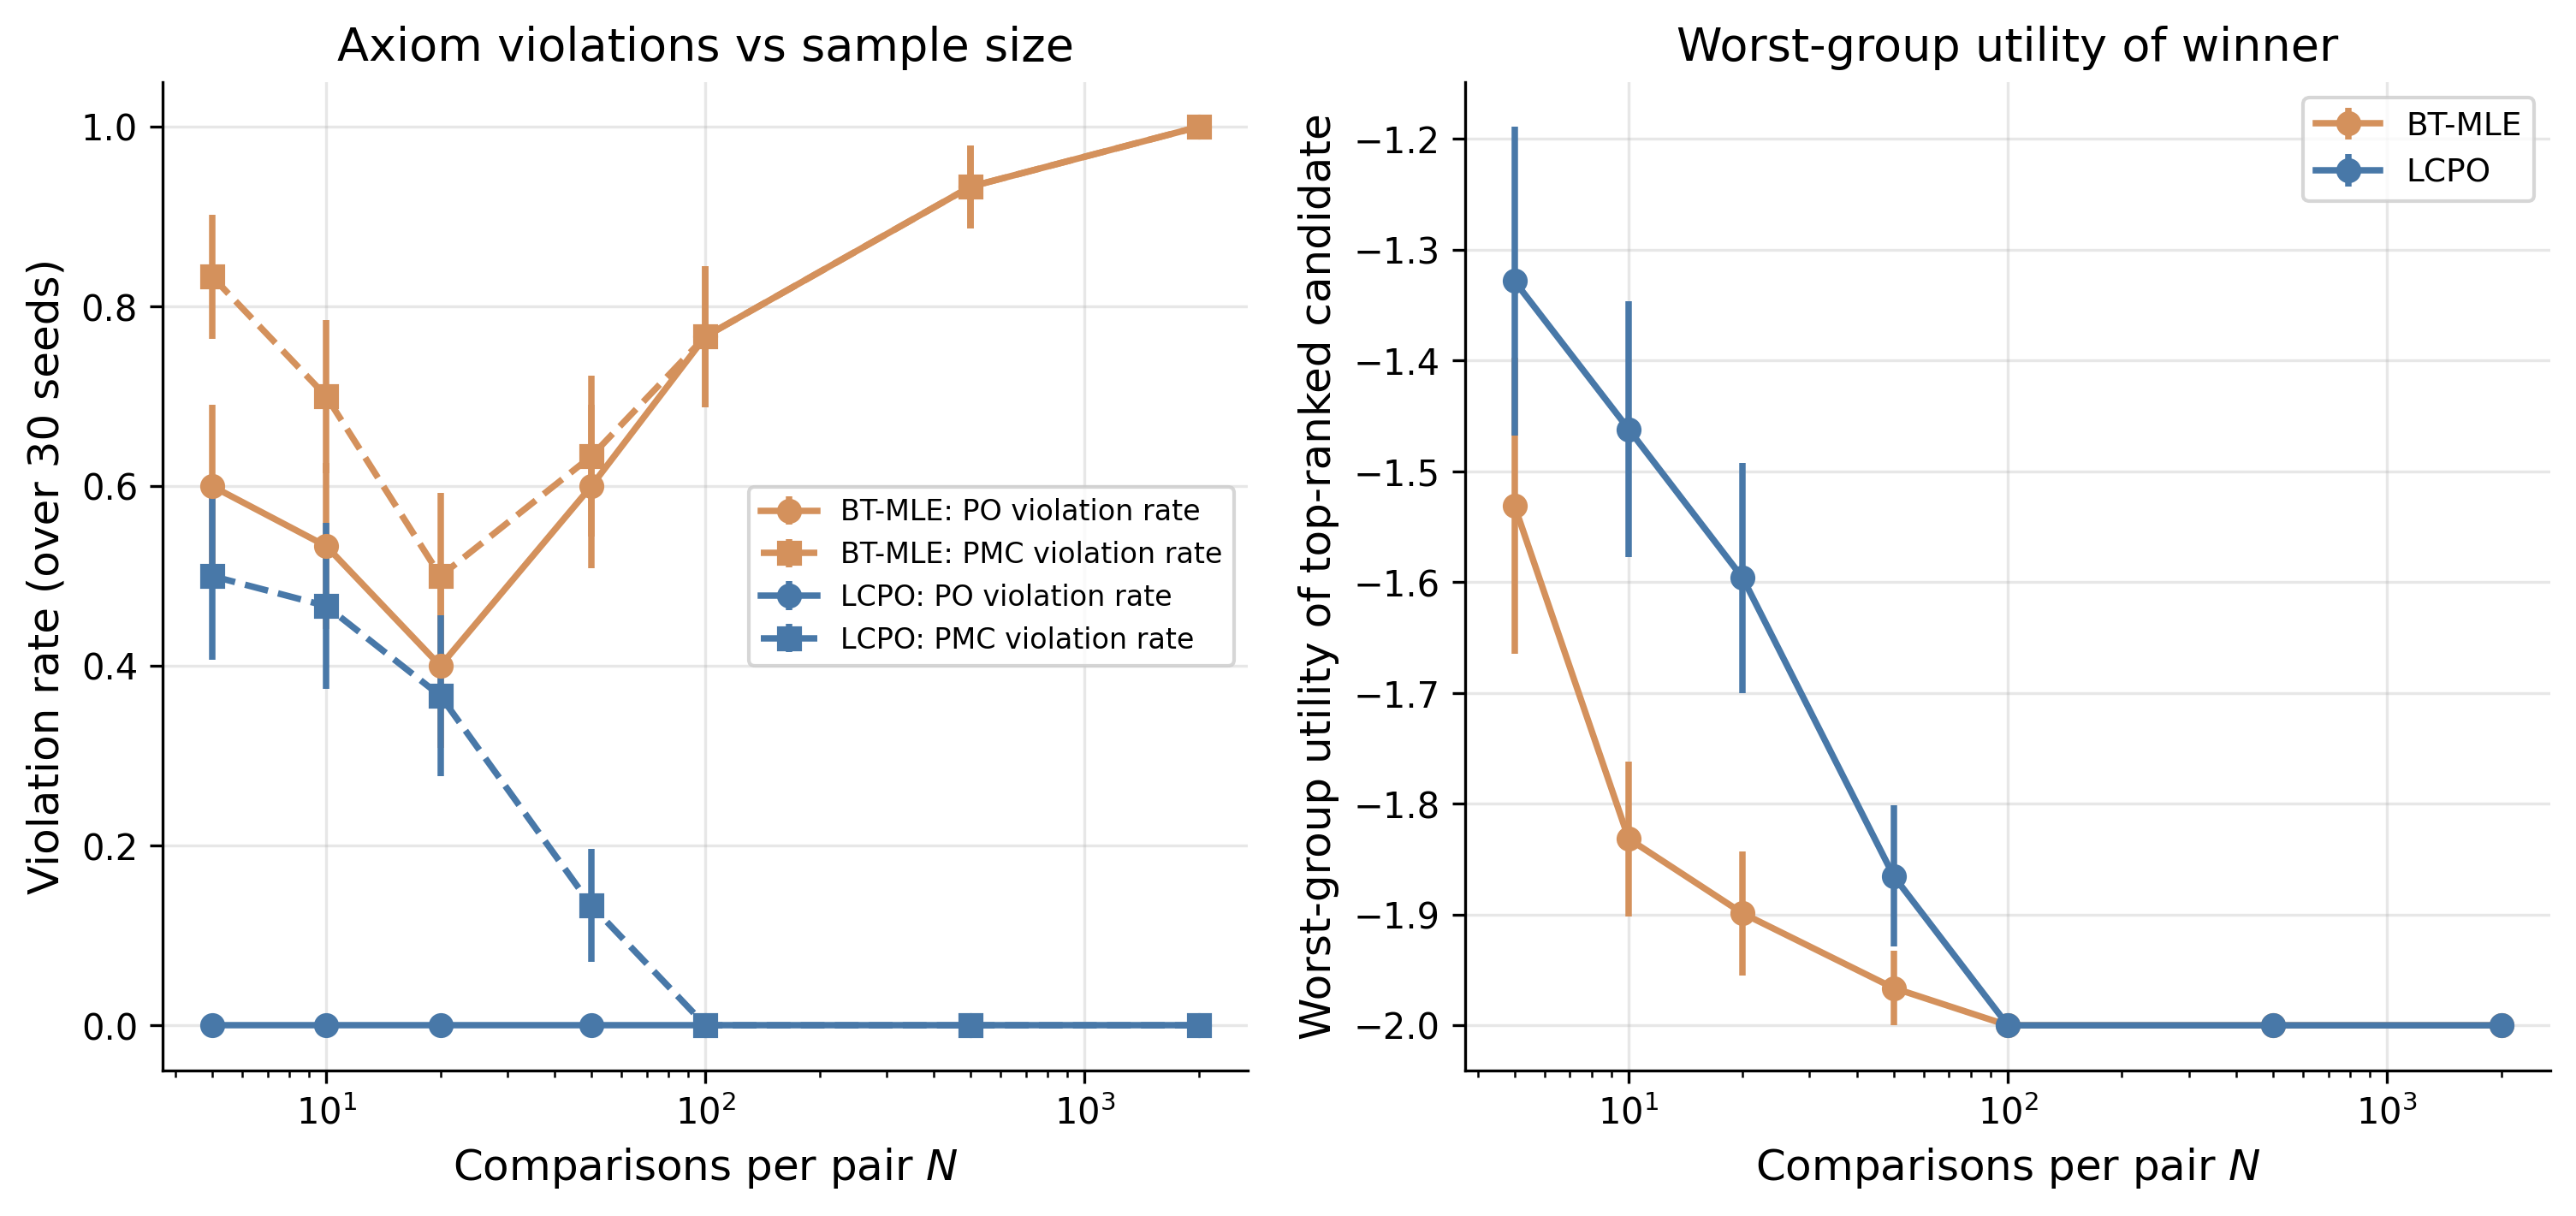
\includegraphics[width=\textwidth]{../ch09_rlhf/sims/axiom_aware_aggregation.png}
\caption[Axiom violation rates and worst-group utility versus sample size]{Axiom violation rates (left) and worst-group utility of the top-ranked candidate (right) versus pairwise comparisons per pair $N$, mean and one standard error over thirty seeds. BT-MLE PO and PMC violation rates rise to one as $N$ grows, in line with Theorem~\ref{thm:bt_mle_failure}; LCPO violation rates remain at zero (PO by construction) or fall to zero (PMC by $N = 100$).}
\label{fig:axiom_aware_aggregation}
\end{figure}

\begin{table}[htbp]
\centering
\caption[Aggregator comparison at $N=2000$ comparisons per pair]{Aggregator comparison at $N = 2000$ comparisons per pair, mean and standard error over thirty seeds. PO viol. and PMC viol. are fractions of seeds on which the output ranking violates the corresponding axiom. Worst-group util. is the type-two utility of the top-ranked candidate. Modal top names the candidate most frequently ranked first.}
\label{tab:axiom_aware_aggregation}
\begin{tabular}{lcccc}
\hline
Method & PO viol. & PMC viol. & Worst-group util. & Modal top \\
\hline
BT-MLE (linear) & 1.00 (0.00) & 1.00 (0.00) & -2.000 (0.000) & a \\
Leximax Copeland (LCPO) & 0.00 (0.00) & 0.00 (0.00) & -2.000 (0.000) & a \\
\hline
\end{tabular}

\end{table}

Figure~\ref{fig:axiom_aware_aggregation} and Table~\ref{tab:axiom_aware_aggregation} report the results. By $N = 2000$, BT-MLE violates both PO and PMC on every seed, as Theorem~\ref{thm:bt_mle_failure} predicts asymptotically. LCPO satisfies PO on every seed at every sample size because the rule directly enforces the Pareto-dominance constraints. LCPO also satisfies PMC on every seed by $N = 100$. The worst-group utility of the top-ranked candidate converges to $-2$ for both methods. The simulation therefore verifies the axiomatic difference rather than an efficiency gain for the top-ranked candidate.

\subsection{Simulation Study: Preference Learning in Job Search}

A worker searches for jobs in a labor market with compensating differentials, following a McCall (1970)-style search model. Wages are measured in thousands and take values $w \in \{20,28,38,50,65,82,100,125\}$, while amenities take values $z \in \{0, 1, \ldots, 6\}$ and capture commute quality, flexibility, and job security. The state space has 112 states: 56 searching states in which the worker observes a pending offer $(w_i, z_j)$ and decides to accept or reject, plus 56 employed states $(w_i, z_j)$ in which the worker decides to stay or quit. The offer distribution exhibits compensating differentials, with wage rank and amenity rank negatively correlated ($\rho = -0.74$): high-wage offers cluster with low amenities and vice versa. The worker's true per-period utility is $u(w, z) = \alpha \log(w) + (1 - \alpha) z$ with $\alpha = 0.6$, but this function is unobserved; the worker can only compare career trajectories (``I prefer path A to path B''), exactly as in stated-preference surveys in labor economics. While searching, the worker receives the unemployment benefit $u_b = \alpha \log(b)$ where $b = 28$. Layoffs occur with probability $p = 0.05$ per period, and the discount factor is $\gamma = 0.95$. Dynamic programming gives $V^*(s_0) = 74.13$; the optimal policy accepts 25 of 56 offer types and stays employed at 25 of 56 job types. Preference data is generated by rolling out a uniform random policy from a random searching state. Each rollout produces a career segment of $L = 15$ periods recording states and actions. For each of $K$ comparisons, two independent career segments are generated; the segment with higher cumulative discounted utility under the true (unobserved) utility function is labeled as preferred via the Bradley-Terry model. Figure~\ref{fig:search_env} shows the optimal accept/reject and stay/quit boundaries.

\begin{figure}[htbp]
\centering
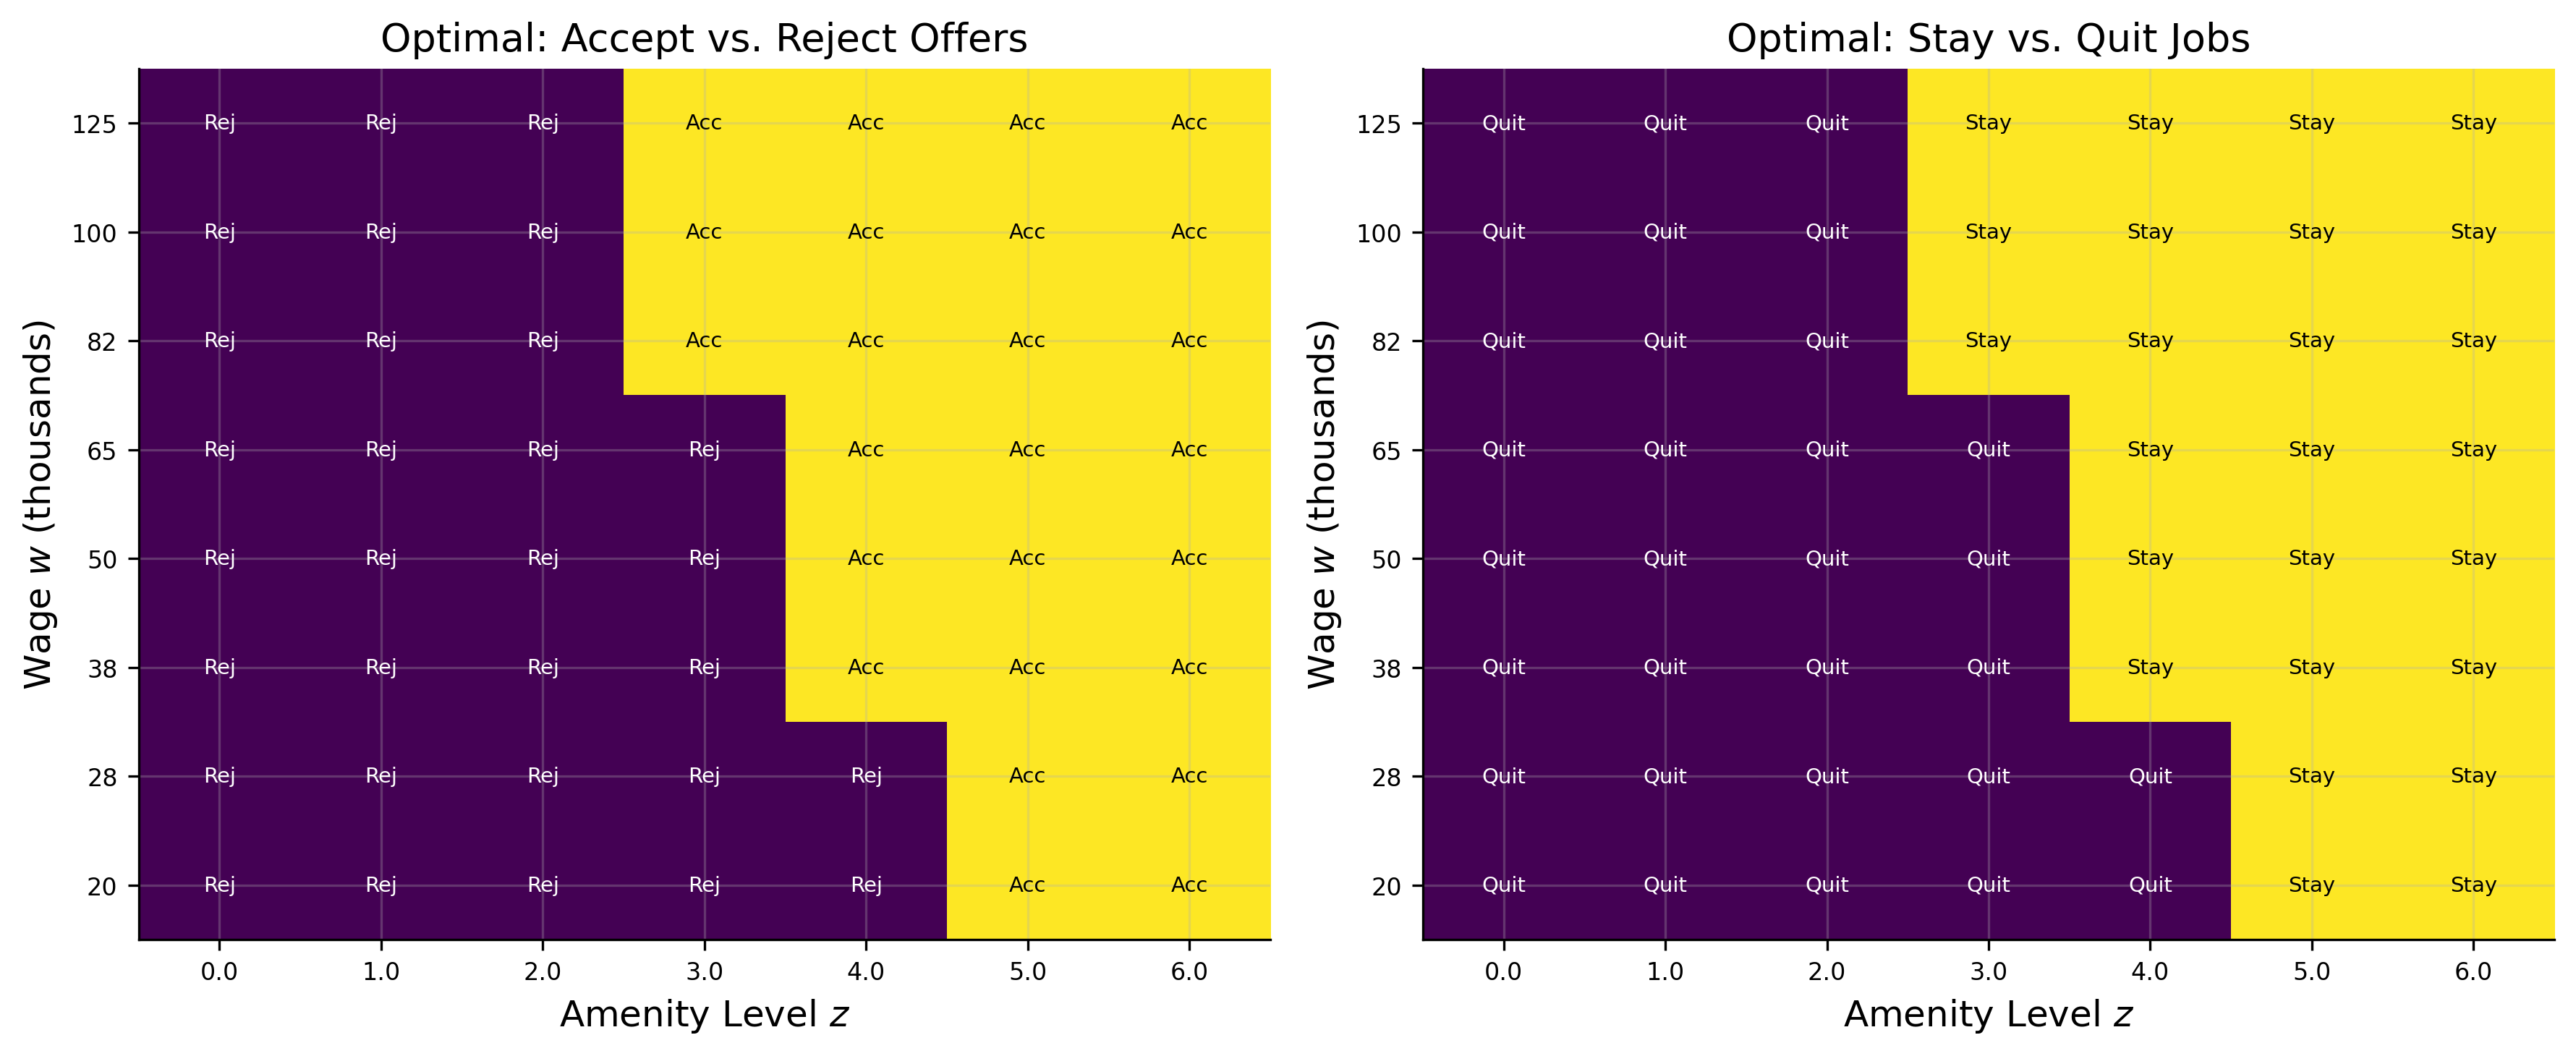
\includegraphics[width=0.85\textwidth]{../ch09_rlhf/sims/job_search_env.png}
\caption[Optimal accept/reject and stay/quit boundaries in wage-amenity space]{Optimal accept/reject and stay/quit boundaries in wage-amenity space. Left: the optimal accept/reject boundary for searching states. Right: the optimal stay/quit boundary for employed states. Both boundaries cut diagonally, reflecting the tradeoff between wage and amenity quality under compensating differentials.}
\label{fig:search_env}
\end{figure}

Six methods are compared across $K \in \{25, 50, 100, 200, 500, 1{,}000, 2{,}000, 5{,}000\}$, averaged over 30 seeds. The neural network RLHF reward model is a two-layer MLP trained by Bradley-Terry MLE on the $K$ segment pairs; per-transition rewards are discount-weighted and summed to obtain a segment score, and the resulting 112-state reward table is solved by value iteration.\footnote{The neural network has 4 inputs (normalized log-wage, normalized amenity, employment indicator, action), 32 hidden units per layer, and $\sim$1{,}200 parameters. The logistic loss from Equation~(\ref{eq:rlhf_loss}) is applied to discount-weighted segment reward sums. The network parameterises $r_\theta(s, a)$, but the table handed to value iteration averages over actions to give $\bar{r}(s) = \tfrac{1}{2}(r_\theta(s, 0) + r_\theta(s, 1))$; this is harmless here because the true per-period reward in this environment is action-independent (actions affect only the next-state transition), so the Bradley-Terry MLE has no incentive to fit action-dependent payoffs.} The correctly specified structural model parameterizes utility as $\hat{u} = \hat{\alpha} \log(w) + (1 - \hat{\alpha}) z$, estimating the single parameter $\hat{\alpha}$ via Bradley-Terry MLE, then solves the MDP. The misspecified model uses $\hat{u} = \hat{\alpha} \log(w) + (1 - \hat{\alpha}) \bar{z}$, where $\bar{z} = 3$ is the mean amenity level; this model ignores amenity variation across jobs, treating all amenities as identical. DPO trains a tabular softmax policy directly from trajectory comparisons, bypassing reward modeling entirely.\footnote{DPO uses 112 logit parameters $\phi_s$, one per state, trained via the DPO loss (Equation~\ref{eq:dpo_loss}) with Adam optimization over a sweep of $\lambda_{KL} \in \{0.01, 0.05, 0.1, 0.5, 1.0, 5.0\}$, selecting the $\lambda_{KL}$ that minimizes training loss. The reference policy is uniform: $\pi^{SFT}(a|s) = 0.5$. To match the LLM setup where both completions condition on the same prompt, DPO comparison pairs start from the same initial state.} Tabular Q-learning ($10{,}000$ episodes, $\varepsilon = 0.15$, learning rate $0.1$) and exact DP provide scalar-reward baselines. All four preference methods receive identical comparison data per seed; DPO receives a same-state variant generated from the same seed.

\begin{figure}[htbp]
\centering
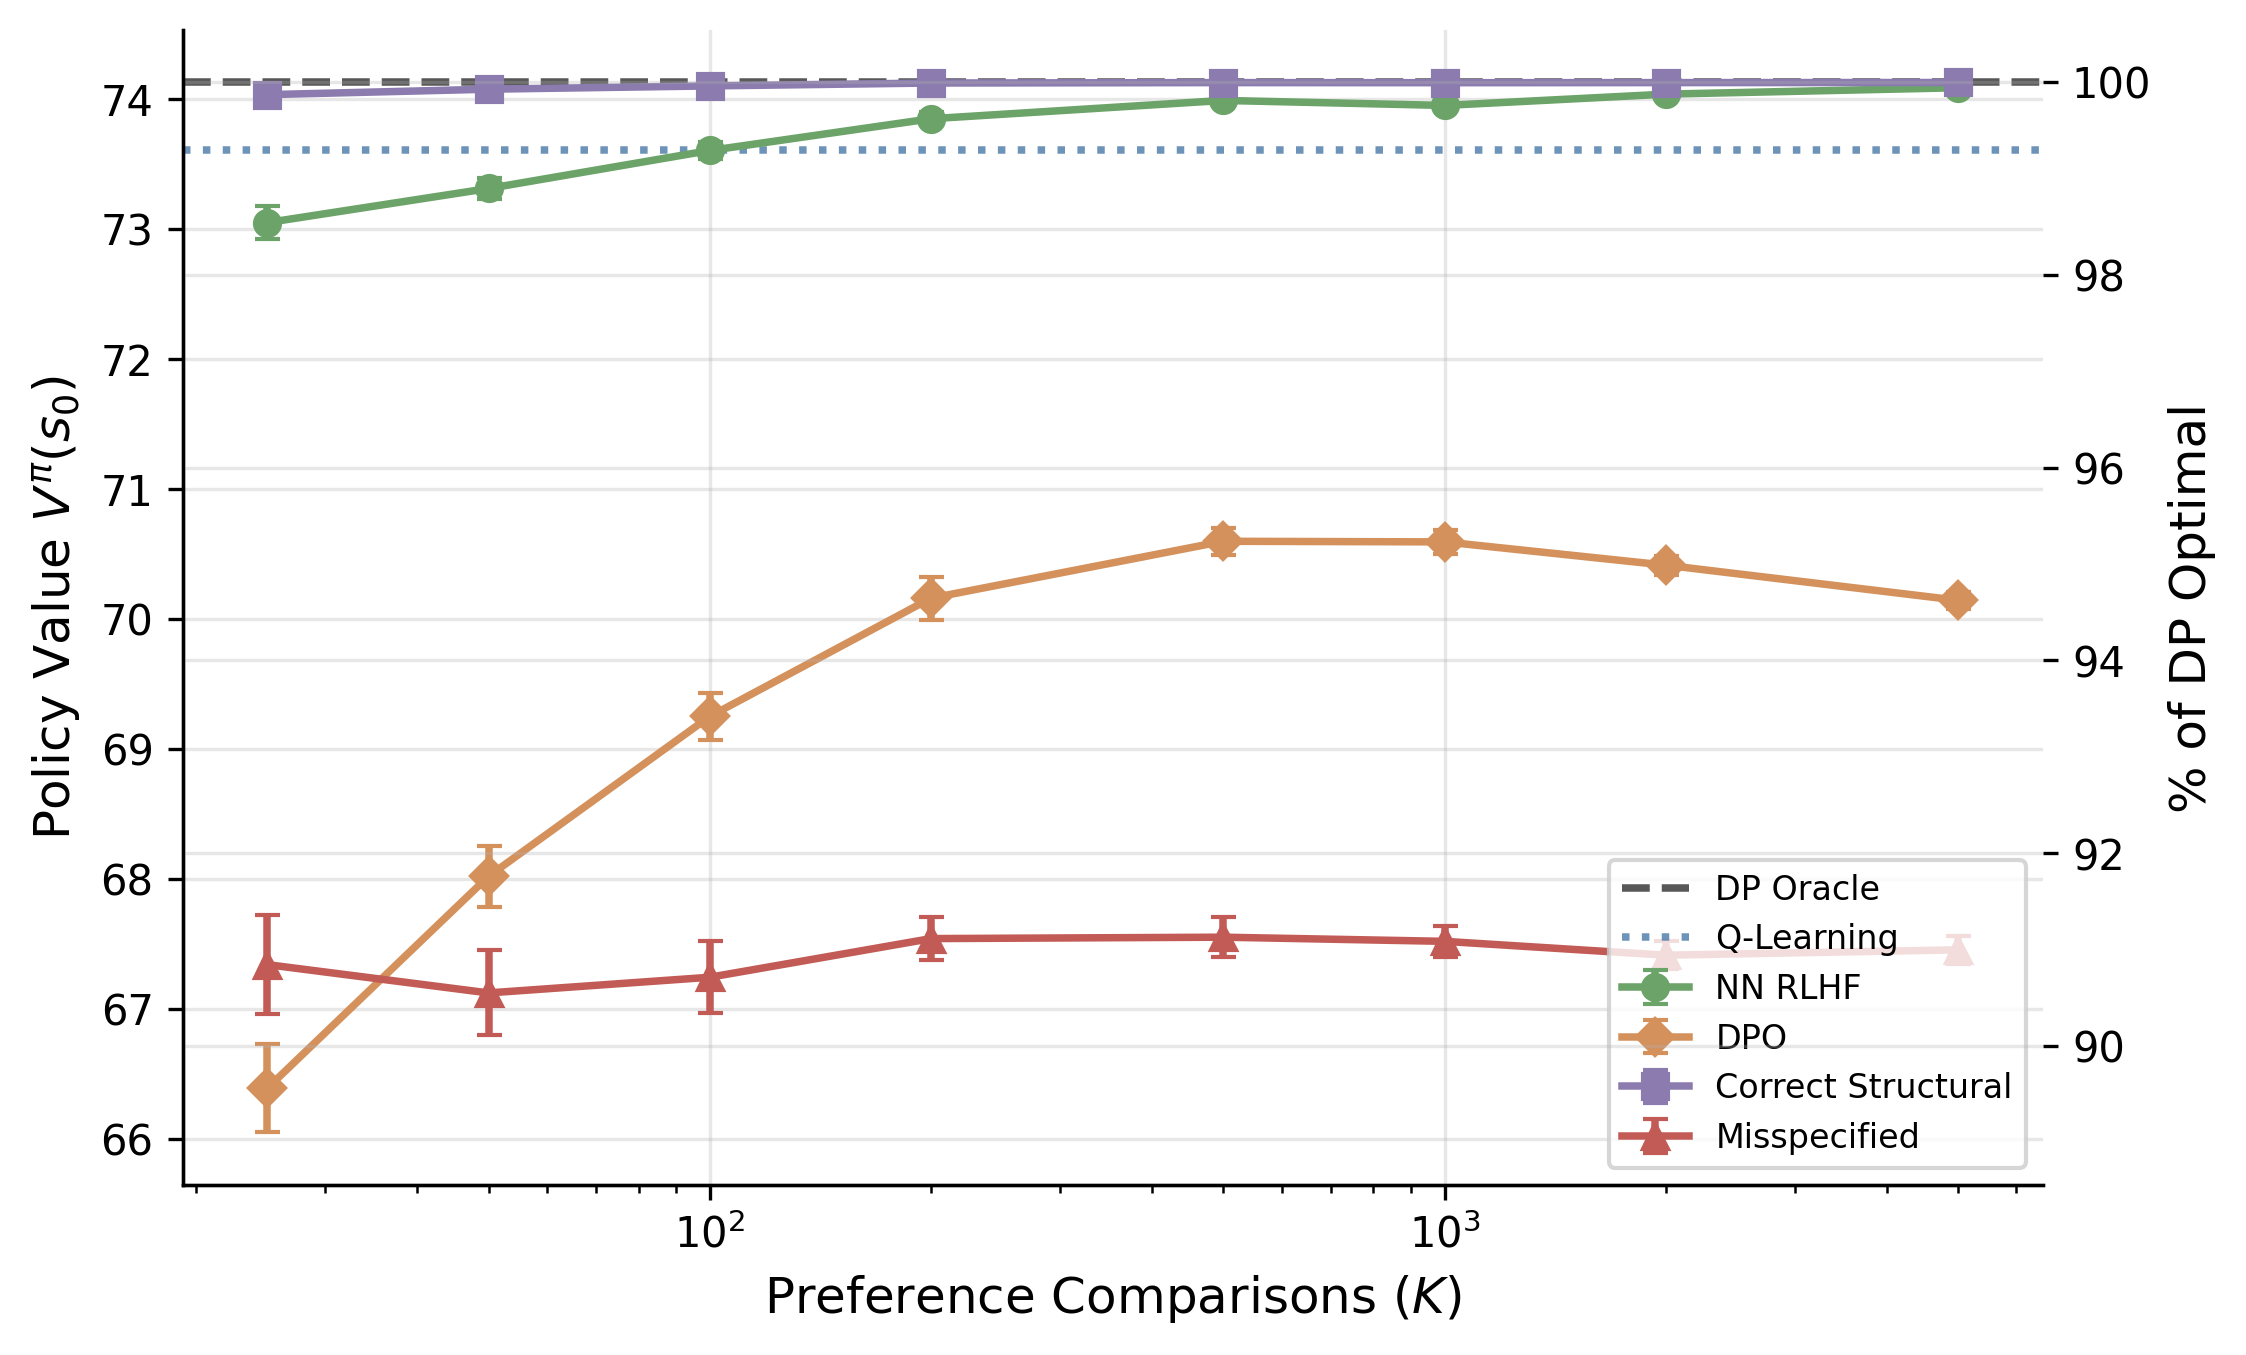
\includegraphics[width=0.7\textwidth]{../ch09_rlhf/sims/job_search_sample_complexity.png}
\caption[Policy value versus number of preference comparisons $K$ for all six methods]{Policy value $V^\pi(s_0)$ versus number of preference comparisons $K$ for all six methods (30 seeds, $L = 15$). The right axis shows the percentage of DP-optimal value.}
\label{fig:preference_sample}
\end{figure}

Figure~\ref{fig:preference_sample} reports the main results. The correctly specified structural model reaches 99.9\% of the DP optimum at $K = 25$. Its one-parameter specification gives the structural model this sample-efficiency advantage. The neural network converges more slowly and reaches 99.9\% by $K = 5{,}000$, consistent with the larger sample requirement of a flexible model. DPO reaches approximately 95\% by $K = 500$ and then plateaus.\footnote{DPO learns only from $(s,a)$ pairs visited in training trajectories generated by the random behavioral policy. It cannot propagate value to undervisited states the way value iteration does after learning a reward model, so states poorly covered by the behavioral policy remain suboptimal regardless of $K$.} The DPO plateau differs from the gridworld result of $-118\%$. DPO recovers a viable job-search policy, but additional data do not close the remaining gap.\footnote{DPO fails catastrophically in gridworld because transitions are stochastic (10\% slip probability) and rewards are transition-dependent. The same $(s,a)$ pair yields different rewards depending on whether the agent slipped, so the DPO loss conflates policy quality with transition luck. In the job search model, accept/reject deterministically changes employment status, and only the 5\% layoff probability introduces stochastic transitions.} The misspecified constant-amenity model remains at 91\% as $K$ grows because additional preference data cannot recover the omitted amenity variation.

\begin{table}[htbp]
\centering
\caption[Diagnostics at $K = 5{,}000$: policy agreement with $\pi^*$, value-function correlation, and mean accepted wage and amenity for each method]{Diagnostics at $K = 5{,}000$ (single seed): policy agreement with $\pi^*$, value-function correlation, and mean accepted wage and amenity for each method.}
\label{tab:preference_diagnostics}
\input{../ch09_rlhf/sims/job_search_diagnostics.tex}
\end{table}

Table~\ref{tab:preference_diagnostics} provides state-level diagnostics at $K = 5{,}000$. The structural model and neural network achieve near-perfect policy agreement with $\pi^*$ (100\% and 96\% respectively). DPO agrees on only 57\% of states with value-function correlation 0.78, systematically underselecting on both wage and amenity dimensions.\footnote{DPO's mean accepted amenity of 3.4 parallels the misspecified structural model's 3.0, though the mechanisms differ: the misspecified model ignores amenity variation by construction, while DPO underweights amenities because the random behavioral policy underrepresents high-amenity employed states in the training data.} The misspecified model agrees on 50\%, with disagreements concentrated where amenity variation matters.\footnote{An online versus offline ablation for the neural network at $K = 1{,}000$ (20 seeds) shows comparable performance: online $73.92 \pm 0.05$, offline $73.99 \pm 0.03$ ($p = 0.09$). The random behavioral policy already provides diverse career trajectories covering the full wage-amenity space.}

\begin{figure}[htbp]
\centering
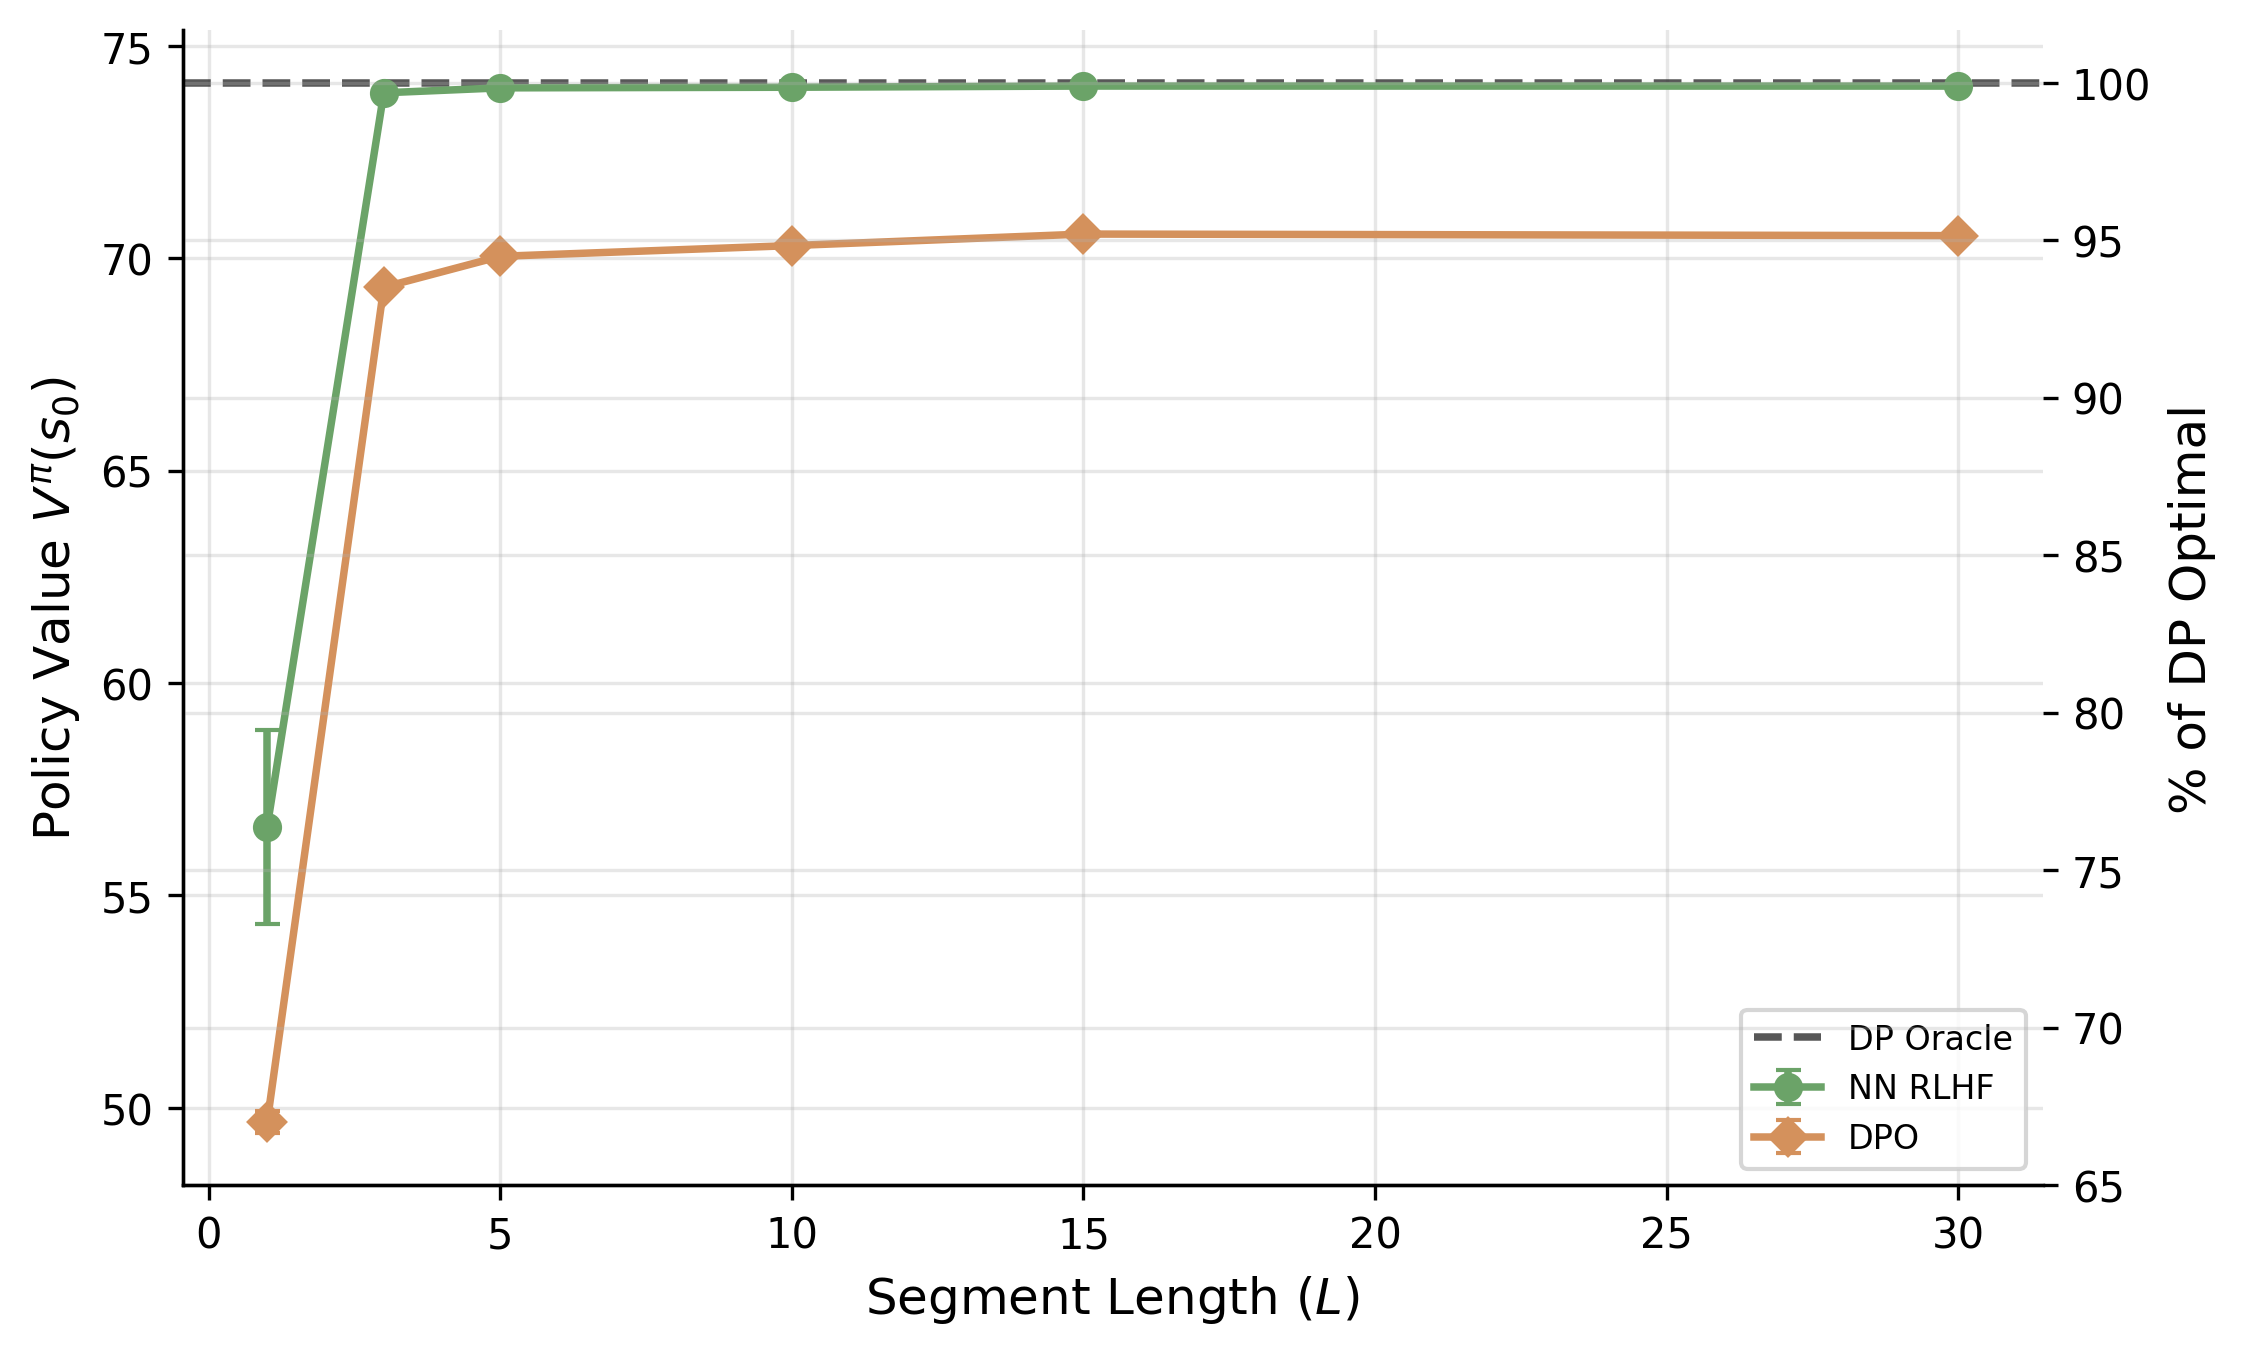
\includegraphics[width=0.7\textwidth]{../ch09_rlhf/sims/job_search_horizon.png}
\caption[Policy value versus segment length $L$ at $K = 2{,}000$ for the neural network and DPO]{Policy value $V^\pi(s_0)$ versus segment length $L$ at $K = 2{,}000$ for the neural network and DPO (20 seeds). The right axis shows the percentage of DP-optimal value.}
\label{fig:preference_horizon}
\end{figure}

Figure~\ref{fig:preference_horizon} reports the segment length ablation at $K = 2{,}000$. At $L = 1$, both methods perform poorly because single-step comparisons carry minimal information about long-run value. The neural network recovers rapidly (by $L = 3$) because the reward model aggregates per-transition estimates over longer segments and value iteration propagates them through the full transition structure; DPO improves monotonically but plateaus at its $\sim$95\% ceiling, as it must learn the policy directly from trajectory comparisons without access to the transition model.

Two-stage RLHF separates preference estimation (a static econometric problem) from dynamic programming (which exploits the known transition model); DPO conflates the two and forfeits the transition structure that structural modelers typically have access to.\footnote{This advantage is specific to settings where the transition model is known or estimable; in domains without a tractable transition model, DPO's single-stage approach avoids compounding errors from reward model estimation.} The DPO plateau in the job-search study is the computational version of the identification point above. More comparisons tighten the empirical binary choice model on the support of observed trajectories, but they do not reveal counterfactual value in poorly covered states, nor do they identify a welfare object independent of the aggregation rule used to construct the labels.
